%
% Documento: Tecnologia de Informação Verde
%

\chapter{Tecnologia da Informação Verde}

\section{Informação}

De acordo com \citeonline{pinheiro2004informaccao}, a informação é dependente de um contexto (científico, tecnológico, industrial, artístico, cultural, entre outros). Segundo \citeonline[p. 17]{aguilar2009tecnologia}, a informação corresponde a grupos de dados classificados e organizados, que tenham valor para que uma pessoa ou empresa consiga utilizá-la em seu benefício. Na vida real ou empresarial, dispor de informação é um fator determinante para o sucesso e seu mal uso pode trazer grandes prejuízos. Para ajudar a resolver esse problema existe o que chama de Tecnologia da Informação (TI).

\section{Tecnologia da Informação}

A evolução humana tem ligação direta com o avanço da tecnologia, bem como o contrário. Um é inerente ao outro e isso é indiscutível quando observamos as várias mudanças nos instrumentos, que se tornaram mais funcionais, acompanhando a evolução do homem, tanto na anatomia de seu corpo, principalmente de sua mão, quanto em seu cérebro. \cite[p. 107-111]{acevedo1998ciencia}. Ela foi desenvolvida para satisfazer as necessidades humanas e já existia antes dos homens e dos conhecimentos científicos e mesmo assim foi capaz de criar estruturas e instrumentos complexos. \cite{acevedo1998ciencia, veraszto2004projeto}. 

Para \citeonline[p. 2]{de1996tecnologia}, a tecnologia pode ser definida como conjunto de conhecimentos, em sua maioria científicos, que são aplicados em determinados ramos de atividades. Podendo ser considerada uma ciência que trata da técnica.

A TI é um dos campos da tecnologia que tomou força no século XX. Surgiu como um meio para melhorar os processos de criação e desenvolvimento \cite[p. 2]{de1996tecnologia}, e atualmente é um forte indicador de melhoria na performance e produtividade \cite[p. 2]{lunardi2001efeitos}, além de ter grande relevância na continuação de esforços das empresas para tornarem os seus processos mais ágeis e produtivos \cite{shaw1997information}. Seu grande papel é o gerenciamento de informações, mas nem sempre esse gerenciamento se dá de forma responsável para o meio ambiente \cite[p. 6-7]{silva2011}. Para apontar soluções aos problemas e amenizar os riscos ambientais decorrentes da Tecnologia de Informação, pesquisadores sugeriram uma série de práticas de Tecnologia da Informação Verde.

\section{Tecnologia da Informação Verde}

O grande avanço tecnológico dos últimos anos, acompanhado da obsolescência programada dos produtos, apresentada por \citeonline{bulow1986economic}, e do consumo desenfreado com consequente produção em grande escala resultam em grandes riscos para o meio ambiente. O descarte inadequado do Resíduos de Equipamentos Eletroeletrônicos (REEE) tem grande impacto ambiental e traz sérios riscos à saúde humana, sendo uma das causas da contaminação de solos e águas com minérios pesados. Há também o grande gasto de energia, uma vez que o número de aparelhos eletrônicos vem crescendo em empresas e indústrias além de vários serviços que são utilizados 24 horas por dia ou são atualizados sempre, impedindo seu desligamento durante a noite ou fins de semana.

Segundo \citeonline[p. 2]{laurindo2000estudo}, a tecnologia “não só sustenta as estratégias de negócio existentes, mas também permite que se viabilizem novas estratégias empresariais”. Uma dessas novas estratégias surgiu com a busca pela redução dos impactos ambientais e a possível reversão de danos causados, o que resultou no estabelecimento de práticas sustentáveis na área de TI, que juntas são conhecidas como TI Verde. \cite{aguilar2009tecnologia}.

A TI Verde vem do conceito de ecoeficiência, e teve origem na década de 80. Consiste do uso eficiente dos recursos naturais, e atualmente vem sendo utilizado com frequência nos setores de TI. \cite{ferreira2009tiverde}. Atualmente, a TI Verde pode ser definida como um conceito que as empresas de tecnologia criaram para agregar o uso de recursos tecnológicos e políticas que minimizem cada vez mais as agressões ao meio ambiente. \cite{briefing2008preciso}.

\begin{citacao}
É o estudo e a prática de projetar, fabricar, usar e descartar computadores, servidores e subsistemas associados, como monitores, impressoras, dispositivos de armazenamento e sistemas de rede e comunicação, de maneira eficiente e eficaz, com impacto mínimo ou nenhum impacto no ambiente. A TI Verde também se esforça para alcançar a viabilidade econômica e melhorar o desempenho e uso do sistema, respeitando nossas responsabilidades sociais e éticas \cite{murugesan2008harnessing}.
\end{citacao} 

Para \citeonline[p. 36]{aguilar2009tecnologia}, a economia de energia e o corte de gastos sempre foram as grandes preocupações das empresas. Essa preocupação se torna ainda maior na área de TI, pois os \textit{datacenters} geralmente costumam figurar como a maior porcentagem dos gastos de energia elétrica de uma companhia, já que em um banco, por exemplo, a energia que a TI utiliza pode superar a metade de todo consumo.  

Além da preocupação com o meio ambiente, várias dessas práticas têm um impacto econômico positivo, o que contribui para sua ampla adoção, já que a busca pelo aumento da produtividade passa pela redução de gastos e tem influência direta da utilização de recursos básicos, como água, energia e matérias primas.

\section{Tecnologia da Informação Verde nas organizações}

Para \citeonline{kraemer2005responsabilidade} o fator ambiental vem mostrando a necessidade de adaptação das organizações e consequentemente direcionando novos caminhos na sua expansão. As organizações precisam alterar seus paradigmas, mudando sua visão empresarial, objetivos, estratégias de investimentos e de marketing, se adaptando à nova realidade do mercado global e ecologicamente correto.

\begin{citacao}
As empresas têm um papel extremamente relevante. Através de uma prática empresarial sustentável, provocando mudança de valores e de orientação em seus sistemas operacionais, estarão engajadas à ideia de desenvolvimento sustentável e preservação do meio ambiente \cite[p. 3]{kraemer2005responsabilidade}. 
\end{citacao}

Os desequilíbrios sócio-ambientais são o resultado do velho paradigma cartesiano e mecanicista, com sua visão fragmentada do mundo \cite[p. 28]{almeida2002bom}. Este paradigma é meramente capitalista e visa o lucro máximo, fazendo com que o meio ambiente seja apenas um bem privado, no que se refere à produção e descarte dos seus resíduos. Este modelo não é sustentável ao longo do tempo, pois ficou claro que os recursos naturais são esgotáveis e, portanto, finitos, se mal utilizados \cite{kraemer2005responsabilidade}.

A \autoref{tab:cartesiano-sustentabilidade} apresenta uma comparação do paradigma atual com o paradigma sustentável.

\begin{table}[htb]	
    \ABNTEXfontereduzida
	\Caption{\label{tab:cartesiano-sustentabilidade} Paradigma cartesiano \textit{versus} paradigma sustentável.}
	\UECEtab{}{
		\begin{tabular}{p{7cm}p{8cm}}
			\toprule
    		\textbf{Cartesiano} & \textbf{Sustentável} \\
			\midrule \midrule
				Reducionista, mecanicista, tecnocêntrico  & Orgânico, holístico, participativo \\
				Fatos e valores não relacionados & Fatos e valores fortemente relacionados \\
				Preceitos éticos desconectados das práticas & Ética integrada ao cotidiano \\ cotidianas &  \\
				Separação entre o objetivo e o subjetivo & Interação entre o objetivo e o subjetivo \\
				Seres humanos e ecossistemas separados, em uma relação de dominação & Seres humanos inseparáveis dos ecossistemas, em uma relação de sinergia \\
				Conhecimento compartimentado e empírico  & Conhecimento indivisível, empírico e intuitivo \\
				Relação linear de causa e efeito & Relação não-linear de causa e efeito \\
				Natureza entendida como descontínua, o todo formado pela soma das partes  & Natureza entendida como um conjunto de sistemas inter-relacionados, o todo maior que a soma das partes \\
				Bem-estar avaliado por relação de poder & Bem-estar avaliado pela qualidade das inter-relações \\ (dinheiro, influência, recursos)  & entre os sistemas ambientais e sociais \\
				Ênfase na quantidade (renda per capita) & Ênfase na qualidade (qualidade de vida) \\
				Análise & Síntese \\
				Centralização de poder & Descentralização de poder \\
				Especialização & Transdisciplinaridade \\
				Ênfase na competição & Ênfase na cooperação \\
				Pouco ou nenhum limite tecnológico  & Limite tecnológico definido pela sustentabilidade \\
			\bottomrule
		\end{tabular}
	}{
		\Fonte{\citeonline{almeida2002bom}}
    }
\end{table}

\subsection{Responsabilidade Social Empresarial}

O Governo vem pressionando cada vez mais as organizações para que desenvolvam práticas a fim de reduzir seus impactos ambientais e sociais. Recentemente, houve grandes progressos quanto à conscientização sobre a responsabilidade social e maior compreensão dos desafios da sustentabilidade \cite{kraemer2005responsabilidade}.

A Responsabilidade Social Empresarial (RSE) pode ser conceituada por meio da integração das preocupações sociais e ambientais em suas operações e interação com todas as partes interessadas. É caraterizada pela sua adoção voluntária, para além das prescrições legais. Este conceito é associado com o de desenvolvimento sustentável, onde as organizações integram em suas operações o impacto econômico, social e ambiental \cite{biorumo}.  

\citeonline{elkington2001canibais} apresenta o termo \textit{Triple Bottom Line}, que também é conhecido como os 3 Ps da sustentabilidade que, segundo \citeonline{biorumo}, são os três fatores fundamentais da RSE:  o planeta, em inglês \textit{planet}, que são as preocupações ambientais, as pessoas, em inglês \textit{people}, que são as preocupações sociais e por último a rentabilidade, em inglês \textit{profit}, que são as preocupações econômicas. Esta tridimensionalidade é representada na figura \autoref{fig:triple_bottom_line}.


\begin{figure}[htb]
    \caption{\label{fig:triple_bottom_line}\textit{Triple Bottom Line}.}
    \begin{center}
        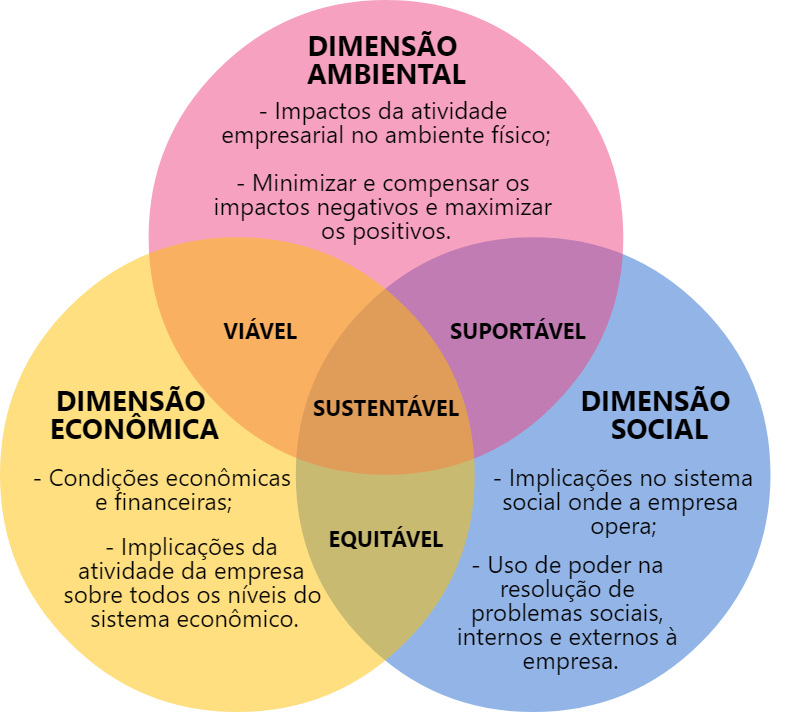
\includegraphics[scale=0.4]{imagens/triple-bottom-line.png}
    \end{center}
    \FonteFigura{Adaptado de \citeonline[p. 24]{biorumo}.}
\end{figure}

\subsection{Sistema de Gestão Ambiental}

\citeonline[p. 103]{nascimento2012gestao} e \citeonline[p. 1082]{tinoco2006contabilidade} definem um Sistema de Gestão Ambiental (SGA) como o conjunto de procedimentos que inclui a estrutura organizacional, atividades de planejamento, responsabilidades, práticas, conjunto de procedimentos, processos e recursos para desenvolver, implementar, atingir, analisar e manter a política ambiental, diminuindo os impactos ambientais de suas atividades, produtos, e/ou serviços.

Algumas atividades que as organizações podem implementar são: estratégias de administração para o meio ambiente; programas de prevenção à poluição; monitorar o programa ambiental da empresa; corrigir os danos ambientais; e adequar os produtos às especificações ecológicas \cite{tinoco2006contabilidade}. O SGA é baseado no cumprimento da legislação ambiental e na melhoria do desempenho ambiental, não basta estar dentro da lei, deve-se sempre melhorar o desempenho com relação ao meio ambiente \apud{nascimento2012gestao}{para2000reduzindo}.

A \autoref{tab:gestao_ambiental} apresenta uma visão geral da gestão ambiental, especificando aspectos da gestão de processos, gestão de resultados, gestão de sustentabilidade e da gestão do plano ambiental.

\begin{table}[htb]
    \ABNTEXfontereduzida	
	\Caption{\label{tab:gestao_ambiental}Visão geral da gestão ambiental.}
	\UECEtab{}{
		\begin{tabular}{llll}
			\toprule
    		\textbf{Gestão de} & \textbf{Gestão de} & \textbf{Gestão de} & \textbf{Gestão do plano} \\
    		\textbf{processos} & \textbf{resultados} & \textbf{sustentabilidade} & \textbf{ambiental} \\
			\midrule \midrule
				Exploração de recursos & Emissões gasosas & Qualidade do ar & Princípios e \\ & & & compromissos \\
				Transformação de & Efluentes líquidos & Qualidade da água & Política ambiental \\ recursos & & & \\
				Acondicionamento de & Resíduos sólidos & Qualidade do solo & Conformidade legal \\ recursos & & & \\
				Transporte de recursos & Particulados & Abundância e & Objetivos e metas \\ & &  diversidade da flora & \\
				Aplicação e uso de & Odores & Abundância e & Programa ambiental \\ recursos & &  diversidade da fauna & \\
				Quadro de riscos & Ruídos e vibrações & Qualidade de vida do & Projetos ambientais \\ ambientais & & ser humano & \\
				Situações de emergência & Iluminação & Imagem institucional & Ações corretivas e \\ & & & preventivas \\
			\bottomrule
		\end{tabular}
	}{
		\Fonte{Adaptado de \citeonline{macedo1994gestao}.}
    }
\end{table}

\section{As práticas de TI Verde}

%As práticas de TI Verde, nos dias atuais, são utilizadas como estratégias de negócio na maior parte das grandes das empresas. Elas garantem lucros, bem-estar e reconhecimento da empresa, além de ajudar na proteção do meio ambiente, melhorando o futuro das próximas gerações, tornando-se imprescindível no dia a dia de qualquer empresa.%

A adoção de práticas sustentáveis é bem vista e traz maior reconhecimento para as organizações que as utilizam, pois, a sociedade atual se preocupa com a preservação do meio ambiente. \cite{abreu2012ti}. Essas práticas são aplicadas de acordo com cada perfil de organização. Nos dias atuais, é indispensável uma análise estrutural da empresa para identificar qual prática mais se adéqua a sua realidade. A implementação dessas práticas trará benefícios tanto para o meio ambiente, como também para a empresa. \cite{pinto2011estudo}.

Estas práticas envolvem ações diversas que têm entre outros objetivos o de economizar recursos naturais e aumentar o tempo de vida útil dos equipamentos eletroeletrônicos. São elas: economia de energia; virtualização de servidores e \textit{desktop}; videoconferência; economia de papel; descarte responsável; e reciclagem de REEE. Com o avanço tecnológico surgiram novas práticas de TI Verde que tornou o uso da TI sustentável \cite[p. 8]{pinto2011estudo}.

\subsection{Os três níveis}

\citeonline{takahashi2009ti} e \citeonline[p. 7]{pinto2011estudo} classificam as práticas de TI Verde em três níveis:

\subsubsection{TI Verde Tático}

Nesse nível as práticas implementadas não modificam a infraestrutura nem interferem nas políticas internas do local, além de não gerarem custos adicionais. Abrangem mudanças ligadas à economia de recursos e tem como medidas o controle do uso excessivo de energia elétrica de uma organização. Alguns exemplos são o monitoramento automático do gasto de energia dos equipamentos, desligando-os quando estão em desuso, o uso de lâmpadas mais eficientes e a mudança na organização e disposição dos equipamentos para melhor circulação e consequente dissipação do calor, otimizando assim a temperatura das salas.

\subsubsection{TI Verde Estratégico}

Nesse nível as mudanças realizadas envolvem a convocação de uma auditoria da infraestrutura de TI e do seu uso relacionado ao meio ambiente e novos meios de produção de bens ou serviços são desenvolvidos e implementados de maneira ecológica. São criadas novas políticas internas e medidas de controle e descarte dos REEE. A adoção destas medidas geram um \textit{marketing} positivo, melhorando assim a imagem dessa organização diante da sociedade. Algumas práticas realizadas neste nível, diferentemente do anterior, geram um custo adicional devido a criação de uma nova rede elétrica visando uma maior eficiência energética e de sistemas computacionais que tenham um menor consumo elétrico, por meio da substituição dos equipamentos por outros mais econômicos e possíveis reformas estruturais.

\subsubsection{TI Verde a Fundo}

Esse nível é a integração dos níveis anteriores. É necessária a criação de um projeto de total modificação estrutural para maximizar a economia de energia e a sustentabilidade da organização. São realizadas grandes mudanças na infraestrutura que visam otimizar o desempenho dos equipamentos e a padronização dos processos, como projetos de sistemas de refrigeração, iluminação, disposição de equipamentos e a possível utilização e fontes de energia limpa ou renováveis, gerando um alto custo para a sua implementação.

\subsection{Virtualização}

A virtualização é uma técnica utilizada para emular um ambiente computacional sobre outro, ela é bastante popular na maioria das organizações, pois reduz o número de máquinas físicas quando se tem uma diversidade de sistemas operacionais. As máquinas virtuais$^{[}$\footnote{Nome dado para ambientes computacionais simulados.}$^{]}$ podem ter múltiplas instâncias em um mesmo \textit{hardware} e incluem as bibliotecas do sistema operacional desejado, proporcionando um uso eficiente do seu poder de processamento e um alto grau de portabilidade. A redução de máquinas físicas implica na queda dos gastos da infraestrutura, como espaço, energia elétrica, cabeamento, refrigeração, suporte e manutenção de vários sistemas \cite[p. 174-175]{carissimi2008virtualizaccao}.

\citeonline[p. 193]{carissimi2008virtualizaccao} e \citeonline[p. 163-165]{neto2015ti} apresentam os seguintes métodos de virtualização descritos pela \textit{Microsoft}:

\begin{itemize} 
    
    \item Virtualização de Servidor: as máquinas virtuais são criadas através de um software onde as mesmas emulam servidores, permitindo a execução dos seus sistemas operacionais de maneira simultânea. Dois ou mais servidores virtuais são emulados em um único servidor físico, otimizando o uso da memória, processamento e armazenamento (\autoref{fig:virt_serv});
           
    \begin{figure}[htb]
    	\caption{\label{fig:virt_serv}Virtualização de Servidor.}
    	\begin{center}
    	    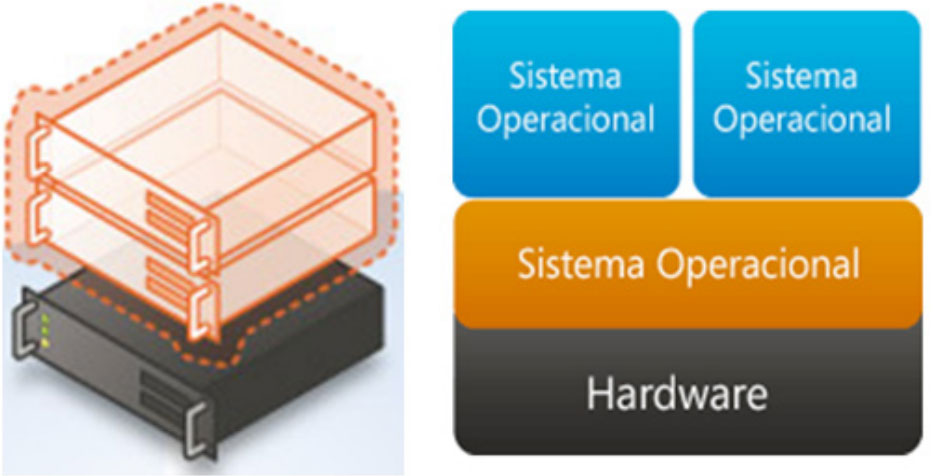
\includegraphics[scale=0.29]{imagens/virtualizacao-servidor.jpg}
    	\end{center}
    	\FonteFigura{\citeonline[p. 163]{neto2015ti}.}
    \end{figure}
    
    \item Virtualização de Estação de Trabalho ou VDI (\textit{Virtual Desktop Infrastructure} - Infraestrutura de estação de trabalho virtual): é utilizado para simular uma máquina virtual "inteira", permitindo o gerenciamento de estações de trabalho com maior eficiência atendendo as necessidades dos usuários. É utilizada para quando existe a necessidade de executar \textit{software} legado$^{[}$\footnote{Termo utilizado para sistemas computacionais que, apesar de serem bastante antigos, fornecem serviços essenciais.}$^{]}$, criar ambientes de testes e treinamento. Cada estação possui seu ambiente com sistema operacional e aplicações independentes. (\autoref{fig:vdi});
    
    \begin{figure}[htb]
    	\caption{\label{fig:vdi}Virtualização de Estação de Trabalho.}
    	\begin{center}
    	    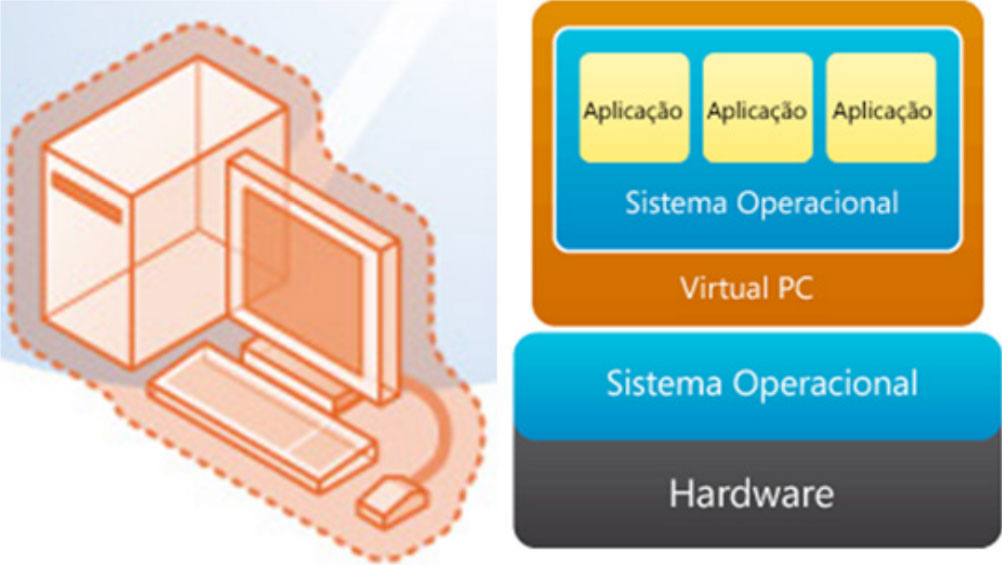
\includegraphics[scale=0.3]{imagens/vdi.jpg}
    	\end{center}
    	\FonteFigura{\citeonline[p. 164]{neto2015ti}.}
    \end{figure}
    
    \item Virtualização de Armazenamento: cria uma camada de abstração entre o sistema operacional e os discos físicos utilizados para armazenamento de dados, permitindo que usuários ou aplicações acessem sem necessidade de informar onde estão localizados ou como é gerenciado (\autoref{fig:virt_arm}).
    
    \begin{figure}[htb]
    	\caption{\label{fig:virt_arm}Virtualização de Armazenamento.}
    	\begin{center}
    	    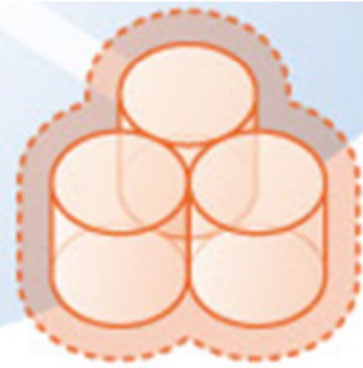
\includegraphics[scale=0.3]{imagens/virtualizacao-armazenamento.jpg}
    	\end{center}
    	\FonteFigura{\citeonline[p. 163]{neto2015ti}.}
    \end{figure}
    
    \item Virtualização de Aplicações: tem como objetivo oferecer aplicações por demanda. A aplicação é alocada em um servidor virtual, que a executa dentro de um próprio ambiente, com isso o usuário não precisa instala-la em sua estação. Cada aplicação fica isolada umas das outras e do sistema operacional subjacente, permitindo ou não a interação e compartilhamento de componentes como dll's$^{[}$\footnote{Sigla para \textit{Dynamic Link Library}, em português Biblioteca de Link Dinâmico, e se trata de uma biblioteca dinâmica que contém dados que podem ser acessados por mais de um programa instalado no computador.}$^{]}$ e \textit{Drivers} (\autoref{fig:virt_apli});

    \begin{figure}[htb]
    	\caption{\label{fig:virt_apli}Virtualização de Aplicações.}
    	\begin{center}
    	    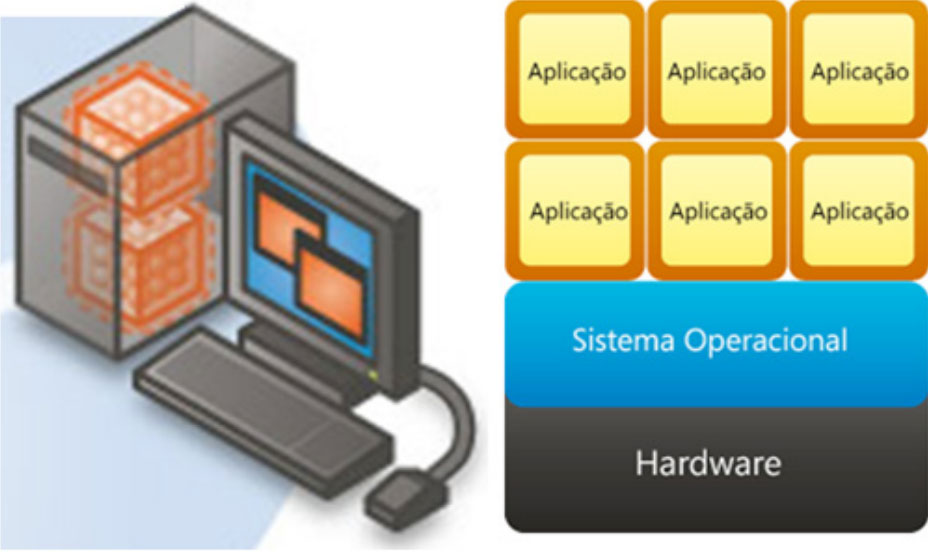
\includegraphics[scale=0.29]{imagens/virtualizacao-aplicacao.jpg}
    	\end{center}
    	\FonteFigura{\citeonline[p. 164]{neto2015ti}.}
    \end{figure} 
    
    \item Virtualização de Apresentação: consiste de um ambiente computacional para acesso à distância, permitindo que uma determinada aplicação seja executada em uma máquina, mas utilize recursos gráficos e de Entrada/Saída de outra e que vários usuários utilizem o sistema não interferindo uns com os outros (\autoref{fig:virt_apre});
    
    \begin{figure}[htb]
    	\caption{\label{fig:virt_apre}Virtualização de Apresentação.}
    	\begin{center}
    	    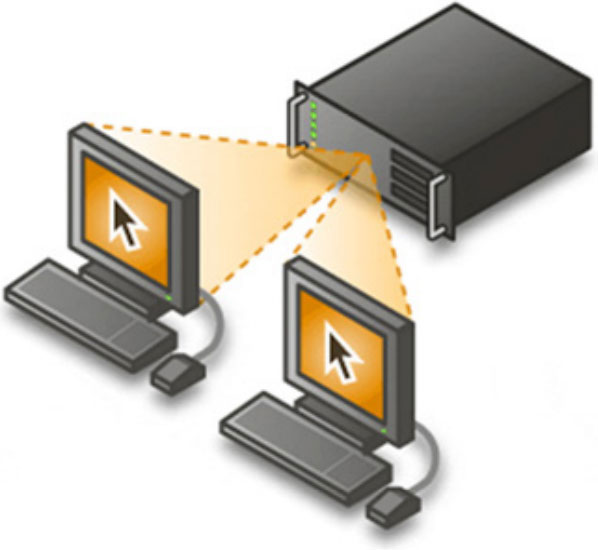
\includegraphics[scale=0.29]{imagens/virtualizacao-apresentacao.jpg}
    	\end{center}
    	\FonteFigura{\citeonline[p. 165]{neto2015ti}.}
    \end{figure}

\end{itemize}

\subsection{Gestão Eletrônica de Documentos}

O Sistema de Gestão Eletrônica de Documentos (GED) foi criado a partir de iniciativas de algumas organizações, como solução para gerenciar a grande quantidade de documentos em forma física \cite{da2003ged}. Segundo pesquisas realizadas pela AIIM$^{[}$\footnote{Sigla para \textit{Association for Information and Image Management}, em português, Associação para a Gestão de Informação e Imagem.}$^{]}$ 92\% das informações dos EUA estavam em papel.$^{[}$\footnote{Informações retiradas do site SEBRAE, Disponível em: \url{http://www.sebrae.com.br/sites/PortalSebrae/ideias/como-montar-uma-empresa-de-administracao-de-arquivos,67f87a51b9105410VgnVCM1000003b74010aRCRD}. Acessado em 17 de julho de 2018}$^{]}$ A sua implantação é de fundamental importância, pois o crescimento exponencial e o acumulo de documentos leva a problemas como a diminuição de espaço físico, perda de documentos, dificuldade de acesso aos documentos e a perca de tempo para localizar os processos \cite{menezes2016ged}.

O GED tem como objetivo aumentar a produtividade, qualidade e agilidade dos processos de informação, armazenando e disponibilizando os documentos digitais e eletrônicos de maneira segura e eficiente \cite{da2003ged}.

Segundo \citeonline[p. 42]{baldam2002ged}, o sistema GED é um conjunto das seguintes tecnologias:

\begin{citacao}
Processamento, arquivamento e recuperação de documentos (Document Imaging); Gerenciamento de documentos (Document Management); Sistema de Gerenciamento de Documentos Técnicos (Engineering
Document Management System); Integração com outros sistemas de processamento de dados (Image Enable); ERM / COLD (Enterprise Report Management) Processamento de formulários (Forms Processing);
Workflow.
\end{citacao}

\citeonline[p. 42]{baldam2002ged} ainda cita outras tecnologias como  ERP (Enterprise Resource Planning), CRM (Costumer Relationship Management), e-Business, Knowledge Management (gerenciamento do conhecimento), PDM (Product Data Management) e EAI (Enterprise Apliccation Integration).


% REEE: Falta refazer e ajustar as informações que eu coloquei aqui. 
\subsection{Resíduos de Equipamentos Eletroeletrônicos}

Resíduos de Equipamentos Eletroeletrônicos é o nome dado a todo resíduo proveniente dos equipamentos eletrônicos \cite[p. 2]{natume2011residuos}. A maioria absoluta desse tipo de resíduo é resultado da obsolescência dos equipamentos eletrônicos, que leva a um descarte de equipamentos antes que esses atinjam seu tempo útil \cite[p. 2]{da2010lixo}. A grande produção de novos aparelhos faz com que os antigos sejam considerados ultrapassados e logo são descartados pelos usuários. Muitas vezes esse descarte é feito de forma inadequada, acarretando assim graves problemas ao meio ambiente.

A \autoref{tab:composicao_fisica} mostra a porcentagem dos principais materiais presentes na composição de um computador, as respectivas porcentagens recicláveis e onde são encontradas.

\begin{table}[htb]	
    \ABNTEXfontereduzida
	\Caption{\label{tab:composicao_fisica} Composição Física de um computador e índice de materiais recicláveis.}
	\UECEtab{}{
		\begin{tabular}{lp{2.6cm}ll}
			\toprule
    		\textbf{Material} & \textbf{\% em relação ao Peso Total}  & \textbf{\% Reciclável}  & \textbf{Localização} \\
			\midrule \midrule
				Alumínio & 14,172 & 80 & Circuito integrado, solda, bateria \\
				%\midrule
				Chumbo & 6,298 & 5 & Semicondutor \\
				%\midrule
				Ferro & 20,471 & 80 & Estrutura, encaixes \\
				%\midrule
				Estanho & 1,007 & 70 & Circuito integrado \\
				%\midrule
				Cobre & 6,928 & 90 & Condutivo \\
				%\midrule
				Bário & 0,031 & 0 & Válvula eletrônica \\
				%\midrule
				Níquel & 0,850 & 80 & Estrutura, encaixes \\
				%\midrule
				Zinco & 2,204 & 60 & Bateria \\
				%\midrule
				Berílio & 0,015 & 0 & Condutivo térmico, conectores \\
				%\midrule
				Ouro & 0,016 & 98 & Conexão, condutivo \\
				%\midrule
				Manganês & 0,031 & 0 & Estrutura, encaixes \\
				%\midrule
				Prata & 0,018 & 98 & Condutivo \\
				%\midrule
				Cromo & 0,006 & 0 & Decoração, proteção contra corrosão \\
				%\midrule
				Cádmio & 0,009 & 0 & Bateria, chip, semicondutor, estabilizadores \\
				%\midrule
				Mercúrio & 0,002 & 0 & Baterias, ligamentos, termostatos, sensores \\
				%\midrule
				Sílica & 24,880 & 0 & Vidro \\
			\bottomrule
		\end{tabular}
	}{
		\Fonte{\url{http://www.tec.abinee.org.br/2007/arquivos/s702.pdf}}
    }
\end{table}

Quando descartados de forma inadequada, em lixões, tem consequências graves ao meio ambiente, como a contaminação de lençóis freáticos e do solo, e às pessoas que entram em contato com esse tipo de lixo, devido aos metais pesados e as peças plásticas presentes nesses aparelhos, que demoram cerca de 150 anos para se decompor no meio ambiente \cite[p. 17]{aguilar2009tecnologia}. 

A \autoref{tab:viloes_eletroeletrônicos} mostra os principais metais usados na composição dos equipamentos eletroeletrônicos e os danos causados em humanos que entram em contato com esses equipamentos. Por isso é necessário que o lixo eletrônico seja descartado de forma correta.

\begin{table}[htb]
    \ABNTEXfontereduzida	
	\Caption{\label{tab:viloes_eletroeletrônicos} Os vilões dos eletroeletrônicos.}
	\UECEtab{}{
		\begin{tabular}{p{2cm}p{3.5cm}p{9cm}}
			\toprule
    		\textbf{Substância} & \textbf{Origem} & \textbf{Efeito} \\
			\midrule \midrule
				Mercúrio & Computador, monitor, televisão de tela plana  & Problemas de estômago, distúrbios renais e neurológicos, alterações genéticas e no metabolismo \\
				%\midrule
				Cádmio & Computador, monitor de tubo e baterias & Agente cancerígeno, afeta o sistema nervoso, provoca dores reumáticas, distúrbios metabólicos e 
				problemas pulmonares \\
				%\midrule
				Zinco & Baterias de celulares e laptops & Provoca vômitos, diarreias e problemas pulmonares \\
				%\midrule
				Manganês & Computador e celular & Anemia, dores abdominais, vômito, seborreia, impotência, tremor nas mãos e perturbações emocionais \\
                %\midrule
                Chumbo & Computador, celular e televisão & Irritabilidade, tremores musculares, lentidão de raciocínio, alucinação, insônia e hiperatividade \\
                %\midrule
                PVC & Usado em fios para & Problemas respiratórios  \\ & isolar corrente & \\
				%\midrule
				Cloreto  & Baterias de celulares e & Acumula-se no organismo e provoca asfixia \\ de Amônia & laptops & \\
				%\midrule
				Arsênio & Celulares & Agente cancerígeno, afeta o sistema nervoso e cutâneo \\
			\bottomrule
		\end{tabular}
	}{
		\Fonte{Adaptado de \citeonline{moi2014lixo}.}
    }
\end{table}

A melhor forma de evitar a contaminação dos humanos é diminuir a geração desse tipo de resíduo, com a manutenção adequadas dos equipamentos existentes além de práticas que aumentem sua vida útil, bem como destinar os resíduos inevitavelmente gerados para um local específico e adequado para tratamento. Deve haver uma preocupação na produção desses equipamentos, cuidando para que a matéria prima seja bem aproveitada e que não haja desperdícios, além de evitar a produção de equipamentos defeituosos, que terão que ser descartados posteriormente.

A \autoref{fig:percepcao} apresenta o ciclo de descarte de um computador, demonstrando a importância de se fazer o descarte adequado, pois além de não poluir o meio ambiente, está prática gera novos mercados e ações de inclusão digital.

\begin{figure}[htb]
	\caption{\label{fig:percepcao}Percepção do problema por mapa conceitual.}
	\begin{center}
	    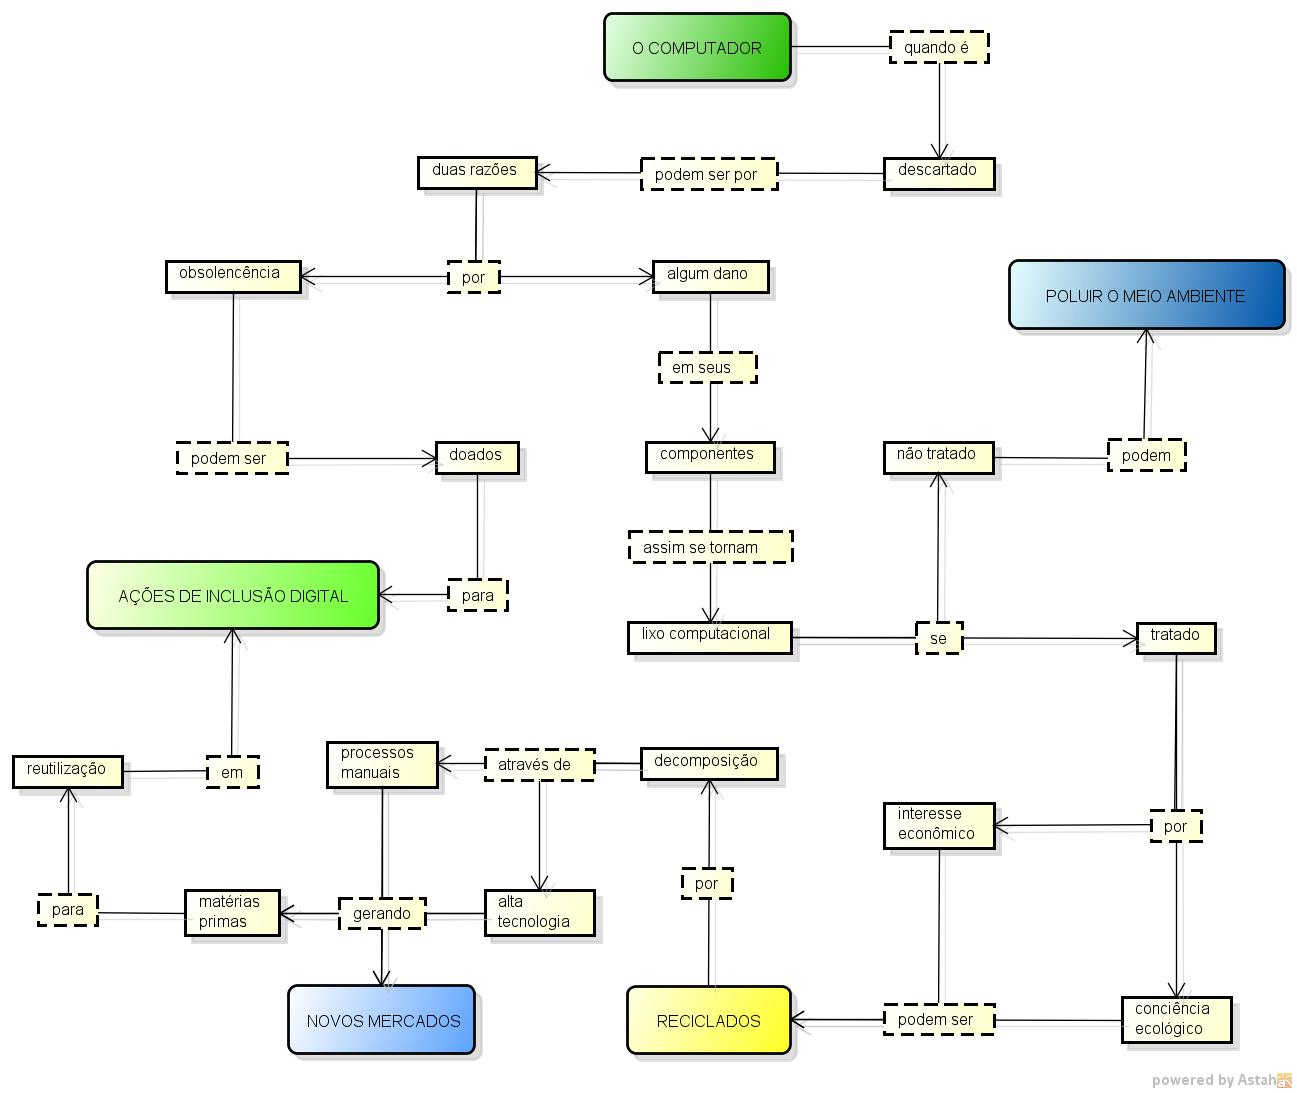
\includegraphics[scale=0.35]{imagens/percepcao-problema.jpg}
	\end{center}
	\Fonte{Adaptado de \citeonline[p. 263]{calvao2009lixo}.}
\end{figure}

% 5R's: Falta revisar, colocar as citações e adaptar melhor.
\subsection{Os cinco R's da educação ambiental}

Os cinco R’s da educação ambiental correspondem a práticas que podem ser implantadas em qualquer lugar e tem impacto que não se limitam ao local em que são aplicados. Estas ações tem como objetivo minimizar a quantidade de REEE, reduzindo na geração de lixo. Estas práticas contribuem na diminuição dos impactos ao planeta, melhorando a vida e contribuindo para o bem estar das futuras gerações. Eles são apresentados pelo \citeonline[p. 35-37]{elementos2009consumo} da seguinte forma:

\subsubsection{Repensar}
Repense e mude os hábitos de consumo e descarte, preferindo sempre adquirir produtos recicláveis ou produzidos de materiais reciclados. Além de praticar ações como a coleta seletiva, evitando o desperdício de alimentos e o uso de produtos biodegradáveis.

\subsubsection{Recusar}
Recusar produtos que prejudicam o meio ambiente e a saúde, comprando apenas produtos que investem na proteção da vida. Se deve evitar excesso de sacolas plásticas, embalagens, lâmpadas fluorecentes, entre outros produtos com embalagens descartáveis e não recicláveis.

\subsubsection{Reduzir}
Reduzir o consumo de produtos e serviços desnecessários, reduzindo os gastos que eles geram, desligando aparelhos eletroeletrônicos quando esses não estão sendo usados. Aqui também entra a preferência por produtos de maior durabilidade e que ofereçam menor potencial de geração de resíduos, impactando na redução no número de produtos consumidos e diminuindo a geração de resíduos.

\subsubsection{Reutilização}
Reutilizar e recuperar ao máximo antes de descartar, ampliando a vida útil dos produtos e dos aterros sanitários. Produtos e embalagens de papel, vidro, plástico, metal, isopor e CDs podem ser reutilizados na criação de produtos artesanais e alternativos. Outra forma é a utilização dos dois lados dos papeis para impressão, montando blocos de papel-rascunho. Trocando e doando objetos que possam servir a outras pessoas ou empresas.

\subsubsection{Reciclar}
Reciclar materiais, reduzindo a pressão sobre os recursos naturais, economizando água e energia, gerando trabalho e renda.
Reciclar materiais contribui para a economia de recursos usados na produção e no tratamento de resíduos, além de contribuir para a não contaminação de solos. O ideal é que haja uma separação conforme o tipo de materiais presentes nos resíduos antes da entrega nos postos de coleta seletiva. Essa prática contribui na geração de emprego e renda para milhares de pessoas.

\section{Normas, Regulamentações e Certificados}

Existem normas e certificações que servem para regulamentar e atestar as práticas de TI Verde internacionalmente e nacionalmente. Alguns exemplos de certificações são: ISO 14001, RoHS, Selo Verde, Energy Star e PROCEL. Essas certificações se referem ao processo de trabalho da TI, tanto para a fabricação, quanto para o uso de equipamentos eletrônicos \cite{pinto2011estudo}. 

\subsection{ISO 14001}

A ISO 14001 consiste de uma norma da série ISO 14000 que possui uma grande importância por estabelecer uma base comum para a gestão ambiental eficaz no mundo inteiro, podendo ser aplicada em qualquer tipo de organização \cite{seiffert2005iso}. Ela é ilustrada na \autoref{fig:iso_14001}. 

\begin{figure}[htb]
	\caption{\label{fig:iso_14001}ISO 14001.}
	\begin{center}
	    
\includegraphics[scale=0.35]{imagens/iso-14001.png}
	\end{center}
	\Fonte{\url{https://www.isointegration.net/iso-consulting-service/iso-14001/}}
\end{figure}

No Brasil ela é aplicada através da norma ABNT NBR ISO 14001 que é aceita internacionalmente e define os requisitos para colocar um  SGA em vigor. Ela regulamenta uma eficiente utilização dos recursos, além da redução dos resíduos gerados, exigindo que as organizações considerem todas as questões ambientais em seus processos. Ela foi revista recentemente, ganhando melhorias fundamentais, como o aumento na relevância do SGA nos processos de planejamento estratégico, maior contribuição por parte da liderança e um compromisso com as iniciativas que impulsionem o desempenho ambiental.$^{[}$\footnote{Informações retiradas do site ABNT, Disponível em: \url{http://www.abnt.org.br/publicacoes2/category/146-abnt-nbr-iso-14001?download=396:introducao-a-abnt-nbr-isso-10014-2015}.  Acessado em 12 de julho de 2018}$^{]}$
    
\subsection{RoHS}

O RoHS (Restriction of Certain Hazardous Substances) ou Restrição de Certas Substâncias Perigosas, também conhecida como a Lei do Sem Chumbo, foi criada em julho de 2006 na União Europeia. Essa foi uma das primeiras leis a pressionarem as fabricantes de TI. Após a criação da RoHS, as empresas, indústrias e importadores passou ter a responsabilidade quanto ao ``ciclo de vida'' dos produtos que são inseridos no mercado de consumo \cite{garcia2015tecnologia}. A \autoref{fig:rohs} exibe o selo RoHS Compliant utilizado nos equipamentos eletrônicos.

\begin{figure}[htb]
	\caption{\label{fig:rohs}RoHS Compliant.}
	\begin{center}
	    
\includegraphics[scale=0.35]{imagens/rohs.jpg}
	\end{center}
	\Fonte{\url{http://www.rohsguide.com}}
\end{figure}

Entretanto existe uma teoria, do reciclável poluidor, que trata a reciclagem desse REEE como algo tão poluente como o descarte em aterros, bem como a teoria da diminuição do ciclo de vida dos componentes eletrônicos, uma vez que a reciclagem dos componentes pode dar origem a produtos com curta vida útil \cite{garcia2015tecnologia}.

\subsection{WEEE}

\begin{figure}[htb]
	\caption{\label{fig:weee}Selo WEEE.}
	\begin{center}
	    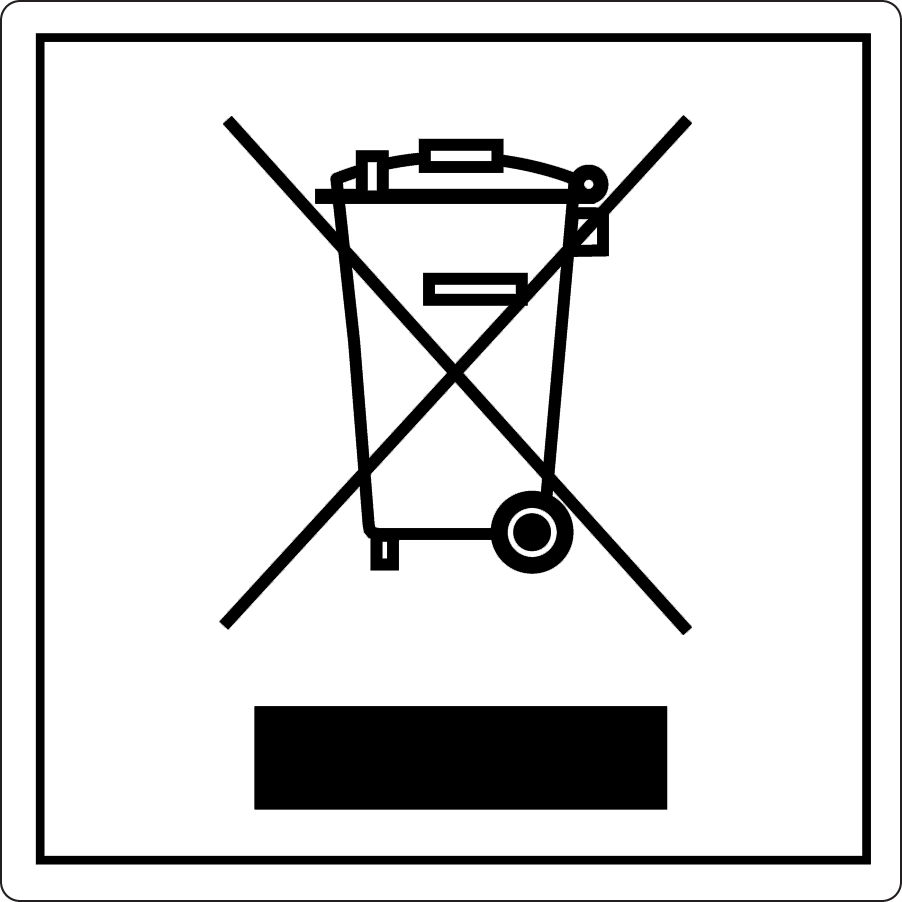
\includegraphics[scale=0.45]{imagens/weee.jpg}
	\end{center}
	\Fonte{\url{https://www.clarionsafety.com/WEEE-Directive/}}
\end{figure}

A WEEE (Waste Electrical and Electronic Equipment Directive) ou Diretiva para o Lixo Elétrico e Equipamentos Eletrônicos também foi criada na Europa com o objetivo de preservar a natureza. Esta diretiva determina o compromisso dos fabricantes com o recolhimento e a destinação correta dos resíduos por eles gerados. A WEEE também prevê a reciclagem, recuperação e reutilização dos resíduos para que estes sejam reduzidos \cite{neto2015ti}. A \autoref{fig:weee} mostra o selo WEEE utilizado nos equipamentos eletrônicos.

\subsection{Selo Verde}

O selo verde é uma forma de reconhecimento de espaços, produtos e serviços que contribuam para a preservação ambiental. Tal selo é atribuído as organizações depois de passarem por um controle de qualidade ambiental. Com isso há o incentivo a promoção de soluções ambientais$^{[}$\footnote{Informações retiradas do site Selo Verde, Disponível em: \url{http://seloverde.org/}.  Acessado em 19 de julho de 2018}$^{]}$, uma vez que os critérios utilizados para certificar uma organização são:  a promoção da conscientização ambiental na comunidade que adquire seus produtos ou serviços; ser economicamente viável e promover a sustentabilidade econômica do ambiente digital; e ser ambientalmente responsável, aplicando os 5R’s em seus processos de forma a produzir com economia de energia ou com pequena quantidade de substâncias tóxicas \cite{abreu2012ti}.

Alguns dos órgãos responsáveis pela aplicação desses selos são: o Greenpeace; o Centro de Computação Eletrônica da Universidade de São Paulo; Instituto da Qualidade Automotiva; e Forset Stewardship Council \cite{pinto2011estudo}.

\subsection{Energy Star}

Energy Star é um programa da U.S. Environmental Protection Agency (EPA) que incentiva a redução na quantidade de energia consumida pelas organizações. Uma de suas práticas é oferecer selos aos fabricantes de equipamentos eletrônicos que optarem pela utilização de tecnologias com funções para poupar energia. A logo da Energy Star está representada na \autoref{fig:energy-star}. 

\begin{figure}[htb]
	\caption{\label{fig:energy-star}Logo do Energy Star.}
	\begin{center}
	    
\includegraphics[scale=0.08]{imagens/energy-star.png}
	\end{center}
	\Fonte{\url{https://www.energystar.gov}}
\end{figure}

\subsection{Procel}

O Selo Procel de Economia de Energia foi criado pelo Programa Nacional de Conservação de Energia Elétrica (Procel), programa instituído por Decreto Presidencial em 8 de dezembro de 1993, sendo desde então executado pela Eletrobras. O objetivo é criar uma identificação para que o consumidor conheça os equipamentos eletrônicos e eletrodomésticos mais eficientes e que consomem menos energia.$^{[}$\footnote{Informações retiradas do site Procel Info, Disponível em: \url{http://www.procelinfo.com.br/main.asp?TeamID={88A19AD9-04C6-43FC-BA2E-99B27EF54632}}. Acessado em 18 de junho de 2018}$^{]}$

\begin{figure}[htb]
	\caption{\label{fig:procel}Etiqueta de Eficiência Energética.}
	\begin{center}
	    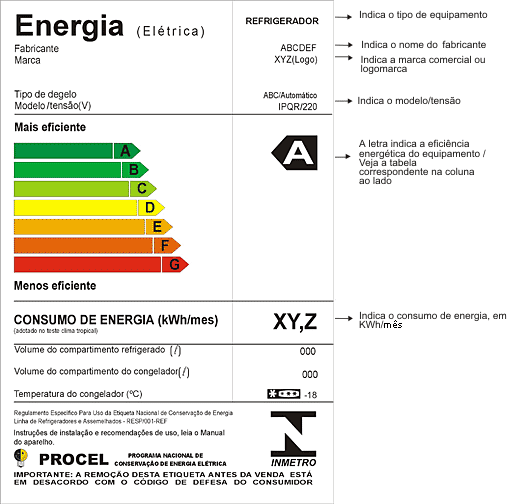
\includegraphics[scale=0.55]{imagens/procel.png}
	\end{center}
	\Fonte{\url{https://goo.gl/sRnNQt}}
\end{figure}

A presença do Selo Procel informa que o equipamento possui uma eficiência energética em sua categoria, já a etiqueta, ilustrada na \autoref{fig:procel}, apresenta algumas informações importantes sobre o equipamento, como os índices de consumo e o desempenho. A observação dessas duas etiquetas contribui para um consumo sustentável de energia.$^{[}$\footnote{Informações retiradas do site iBahia, Disponível em: \url{https://goo.gl/sRnNQt}. Acessado em 18 de julho de 2018}$^{]}$

\subsection{Legislação Brasileira}

O Brasil possui algumas políticas públicas relacionadas à preservação do meio ambiente. As principais são a política federal de saneamento básico, a política nacional de educação ambiental e política nacional de resíduos sólidos.

\subsubsection{Política Nacional de Educação Ambiental} 

A Lei nº 9.785 de 27 de abril de 1999$^{[}$\footnote{Lei nº 9.785 de 27 de abril de 1999, Disponível em: \url{http://www.planalto.gov.br/ccivil_03/LEIS/l9795.htm}. Acessado em 19 de junho de 2018}$^{]}$, também conhecida como política nacional de educação ambiental, é uma lei fundamental no processo de construção da cidadania. O artigo 1º entende a educação ambiental como ``os processos por meio dos quais o indivíduo e a coletividade constroem valores sociais, conhecimentos, habilidades, atitudes e competências voltadas para a conservação do meio ambiente''. Esta lei ainda define políticas públicas que incorporam a dimensão  ambiental, promovendo-a em todos os níveis de ensino, engajando a sociedade quanto a conservação, recuperação e melhoria do meio ambiente.

\subsubsection{Política Federal de Saneamento Básico}

A Lei nº 11.445 de 5 de janeiro de 2007$^{[}$\footnote{Lei nº 11.445 de 5 de janeiro de 2007, Disponível em: \url{http://www.planalto.gov.br/ccivil_03/_ato2007-2010/2007/lei/l11445.htm}. Acessado em 19 de junho de 2018}$^{]}$, regulamenta a prestação de serviços públicos de saneamento básico. Um dos princípios fundamentais dessa lei é a ``utilização de tecnologias apropriadas [...] e a adoção de soluções graduais e progressivas''$^{[}$\footnote{Lei nº 11.445, 5 de janeiro de 2007, Art. 2º VIII}$^{]}$, e uma das diretrizes incentiva o ``desenvolvimento científico e tecnológico, à adoção de tecnologias apropriadas e à difusão dos conhecimentos gerados''.$^{[}$\footnote{Lei nº 11.445, 5 de janeiro de 2007, Art. 48. VIII}$^{]}$ Esta lei também estimula o ``uso de tecnologias modernas e eficientes, compatíveis com os níveis exigidos de qualidade, continuidade e segurança na prestação dos serviços''.$^{[}$\footnote{Lei nº 11.445, 5 de janeiro de 2007, Art. 29.  § 1º  VII}$^{]}$

Segundo o artigo 2º, cabe às empresas, entidades de classe, instituições públicas e privadas, a promoção de ``programas destinados à capacitação dos trabalhadores, visando à melhoria e ao controle efetivo sobre o ambiente de trabalho, bem como sobre as repercussões do processo produtivo no meio ambiente''. Além disso, empresas públicas e privadas devem ser incentivadas, pelo Poder Público, em níveis federal, estadual e municipal, a participarem do desenvolvimento de programas de educação ambiental$^{[}$\footnote{Lei nº 11.445, 5 de janeiro de 2007, Art. 13. Parágrafo único III}$^{]}$ não formal, que tem por objetivo sensibilizar a população em geral sobre as questões ambientais e à sua organização e participação na defesa da qualidade do meio ambiente.

\subsubsection{Política Nacional de Resíduos Sólidos}

No Brasil, a Lei nº 12.305, de 2 de agosto de 2010$^{[}$\footnote{Lei nº 12.30 de 2 de agosto de 2010, Disponível em: \url{http://www.planalto.gov.br/ccivil_03/_ato2007-2010/2010/lei/l12305.htm}. Acessado em 19 de junho de 2018}$^{]}$, institui a Política Nacional de Resíduos Sólidos, dispõe ``sobre seus princípios, objetivos e instrumentos, bem como sobre as diretrizes relativas à gestão integrada e ao gerenciamento de resíduos sólidos, incluídos os perigosos, às responsabilidades dos geradores e do poder público e aos instrumentos econômicos aplicáveis''.$^{[}$\footnote{Lei nº 12.305, 2 de agosto de 2010, Art. 1º  § 1º, p. 1}$^{]}$

Alguns princípios e objetivos da Política Nacional de Resíduos Sólidos são: o desenvolvimento sustentável; a ecoeficiência, visando fornecimento de bens e serviços de um melhor custo-benefício e redução de impactos ambientais; a responsabilidade compartilhada pelo ciclo de vida dos produtos; a proteção da saúde pública e da qualidade ambiental; a aplicação de alguns dos 5R’s, bem como o tratamento adequada dos rejeitos.$^{[}$\footnote{Lei nº 12.305, 2 de agosto de 2010, Art. 6º e 7º}$^{]}$

No que diz respeito a tecnologia da informação, um dos objetivos trata da “adoção, desenvolvimento e aprimoramento de tecnologias limpas como forma de minimizar impactos ambientais.$^{[}$\footnote{Lei nº 12.305, 2 de agosto de 2010, Art. 7º IV}$^{]}$

Uma das diretrizes trata da ordem de prioridade na gestão e gerenciamento de resíduos sólidos: “não geração, redução, reutilização, reciclagem, tratamento dos resíduos sólidos e disposição final ambientalmente adequada dos rejeitos”.$^{[}$\footnote{Lei nº 12.305, 2 de agosto de 2010, Art. 9º}$^{]}$

Os responsáveis pelo destino dos resíduos de eletrônicos são definidos no Art. 33. São eles os fabricantes, importadores, distribuidores e comerciantes de produtos eletroeletrônicos. Eles tem como obrigação “estruturar e implementar sistemas de logística reversa, mediante retorno dos produtos após o uso pelo consumidor, de forma independente do serviço público de limpeza urbana e de manejo dos resíduos sólidos”. Além disso devem “tomar todas as medidas necessárias para assegurar a implementação e operacionalização do sistema de logística reversa sob seu encargo [...], podendo, [...] implantar procedimentos de compra de produtos ou embalagens usados; disponibilizar postos de entrega de resíduos reutilizáveis e recicláveis; atuar em parceria com cooperativas ou outras formas de associação de catadores de materiais reutilizáveis e recicláveis”.$^{[}$\footnote{Lei nº 12.305, 2 de agosto de 2010, Art. 33. § 3º I, II e III}$^{]}$

O Art. 5º diz que a “Política Nacional de Resíduos Sólidos integra a Política Nacional do Meio Ambiente e articula-se com a Política Nacional de Educação Ambiental, regulada pela Lei no 9.795, de 27 de abril de 1999, com a Política Federal de Saneamento Básico, regulada pela Lei nº 11.445, de 2007. Além delas se aplica também aos resíduos sólidos a lei nos 11.445, de 5 de janeiro de 2007, dentre outras normas.$^{[}$\footnote{Lei nº 12.305, 2 de agosto de 2010, Art. 2º}$^{]}$

